\chapter{Divide Areas Algorithm}
\label{chp:DARP}
In this project, the distributed method of multi-robot coverage path planning is implemented. Several different algorithms of this type are discussed in Section \ref{sec:LR Ditributed MCPP}. The algorithm being discussed in this chapter is briefly addressed in Section \ref{sec:LR DARP}. Section \ref{sec:DARP bg} addresses the algorithm in more detail, and Section \ref{sec:DARP dist} discusses the implementation of the algorithm with different distance measures. Section \ref{sec:DARP implement} then goes on to discuss the implementation of this algorithm in the context of this project.
\section{Background Theory}
% TODO: Figure out the subheadings here
\label{sec:DARP bg}
Grid-based coverage path planning can be implemented using a number of different methods. The Voronoi partition method of Section \ref{sec:LR-Voronoi} and the \acl{mstc} method of Section \ref{sec:LR-MSTC} are good examples. Both of these also fall into the distributed category. The \acl{ai} techniques of Section \ref{sec:LR-mAI} and the \acl{mfc} method described in Section \ref{sec:LR MFC} are counter examples of the non-distributed variety.

Naturally, achieving the most optimal solution possible would be most desirable. The authors of the divide areas algorithm described in this section, propose a set of requirements for optimal coverage path planning using a grid-based approach \cite{DARP2017}. These fundamental conditions, as they call them, are listed below.
\begin{enumerate}
\item Every cell in the environment, that is not classified as an object, must be covered. This is known as complete coverage.
\item Each cell in the environment must only be visited once, and only by one of the robots. This is known as the non-backtracking requirement.
\item Each robot should have as close to an equal amount of cells as possible assigned to it for covering. Their sets of cells should be of roughly the same size.
\item The sets of cells assigned to each robot should be a connected sub-region. This means that when generating a path to cover the cells within its set, a robot would not need to traverse the sub-region of another robot to reach its own.
\item The initial position of each robot should be contained within the set of cells assigned to it. This means that a robot would not need to traverse another robot's sub-region to reach its sub-region for coverage.
\end{enumerate}
The authors developed a methodology to achieve these optimal conditions. They called it the \ac{darp}. Their solution seeks to divide a known environment containing static obstacles into contiguous sub-regions. These regions are formed based on the robot starting positions so that each robot starts within one of the regions.

The solution is found in an iterative manner and it converges to where the sub-regions are cohesive and roughly the same size. \ac{darp} only divides the environment appropriately between robots. A single robot \ac{cpp} algorithm can then be utilized to achieve complete coverage of each sub-region, which translates to complete coverage of the whole environment.
% TODO: Maybe mention something about the EXISTENCE of solutions
\subsection{Algorithm Description}
The algorithm works on a two-dimensional environment that is divided into discrete cells. Once the discretisation is complete, the algorithm starts by operating similar to a Voronoi partition. It constructs a matrix for each robot with the same dimension as the environment. The authors refer to these as the Evaluation Matrices ($E_i$). They contain the distances from each cell in the environment to the respective robots. Euclidean distance was used as the distance measure.
\begin{figure}[h!]
\centering
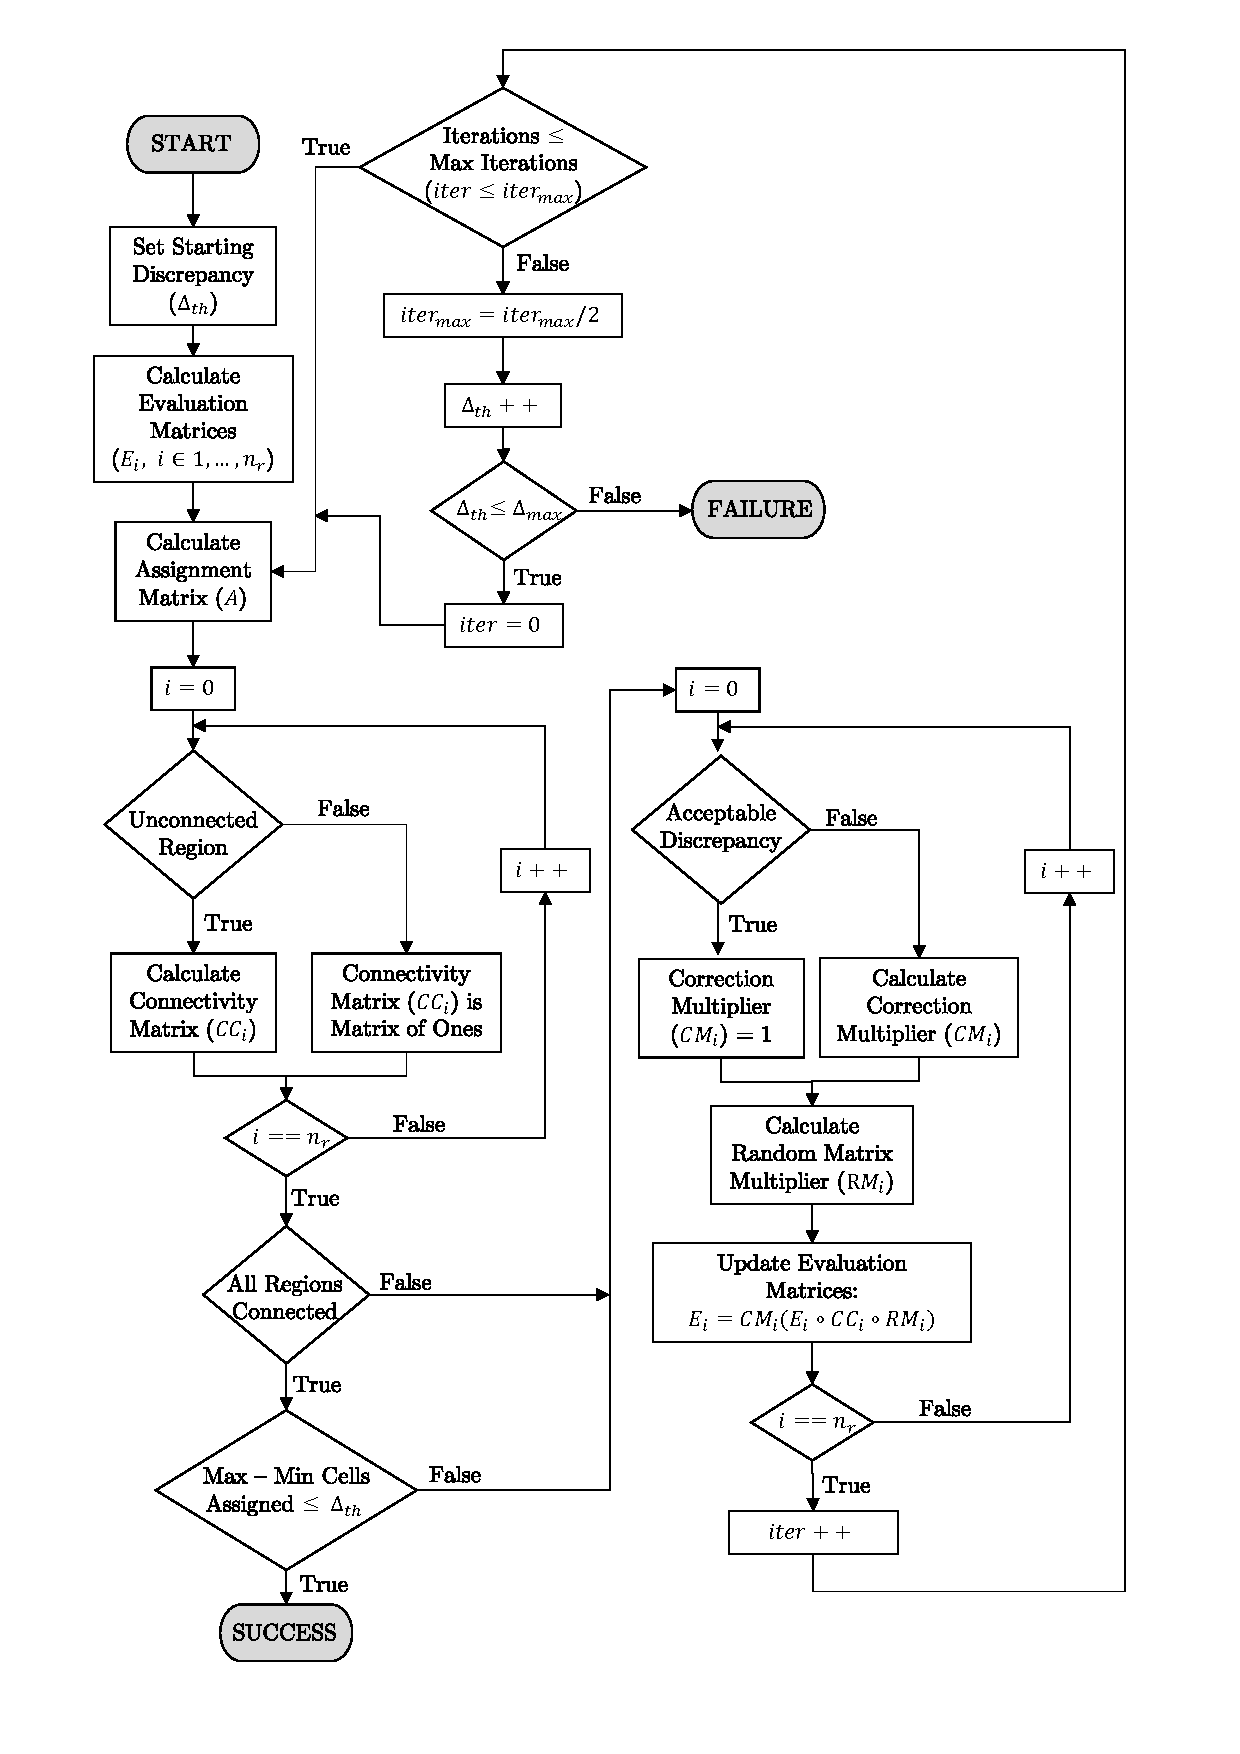
\includegraphics[scale=0.8,trim={1.5cm 0 1.5cm 0},clip]{figs/DARP_Diagram3.pdf}
\caption{Flow diagram representing the logic for DARP.}
\label{fig:DARP}
\end{figure}
\section{Implementation}
\label{sec:DARP implement}
For this implementation, two alterations were made to the \ac{darp} algorithm. The first was a minor change involving an enclosed region checker. The capability was added to detect an enclosed space within the environment and treat it as an obstacle. This change will not be discussed in detail. The second change was adding the ability to use different distance measures, aside from the Euclidean distance measure it was originally implemented with. 

This section has three subsections, starting with a section discussing the suitability of \ac{darp} for this application. The next section goes into detail regarding the different distance measure implementations, and the final section shows some illustrative results where \ac{darp} is implemented in different scenarios.
% TODO: Maybe add section looking at cc and rl values (remember to address section breakdowns then)
% TODO: Mention a bit more about enclosed space handler if you want
\subsection{Algorithm Suitability and Limitations}
% TODO: Add more references - refer back to papers in literature review maybe e.g. online ones for SAR
DARP is a grid-based, distributed , offline algorithm. In this project it has been chosen as an appropriate algorithm in the context of \ac{sar} for a number of different reasons. 
% Why is DARP Appropriate for this problem - grid, offline, distributed

% Grid based
Many existing algorithms make use of a grid-based representation of the environment. In offline approaches, this is convenient to represent the environment. One downside is that if the grid resolution is too low, the representation of the environment becomes less accurate. This is why it is called an approximate approach \cite{Choset2001}. 

The low resolution can be combated by introducing some sensor overlap, or by simply ensuring the resolution is very high. However, higher resolution means more computational power is required, so this should not be done irresponsibly.

% Distributed - justification
Because it is a distributed method, each robot travels only within its allocated sub-region. These regions don't overlap, meaning that the robots will never collide, provided they follow their planned path. Therefore, it removes a layer of complexity that often gets added with multi-robot approaches. So long as the \acp{uav} follow their paths within a reasonable margin of error, they will never collide with one-another.

% Offline - justification (Centralized and decentralized)
It is also an offline approach to \ac{cpp}, so the environment is known prior to the planning phase. The divide areas algorithm and the sub-region coverage algorithm, which is discussed in Chapter \ref{chp:Subregion-Coverage}, are both included in the planning phase. 

Online approaches are generally considered appropriate for dynamic environments. This could refer to any amount of objects in motion within the environment that need to be avoided. Often times, the other \acp{uav} in the environment are modeled as dynamic obstacles from the perspective of a single \ac{uav}. With a distributed approach, this would be unnecessary, because the \ac{uav} paths will never cross one-another. 

Sometimes, online approaches are deemed appropriate because inputting the environment into the planner a priori is considered too costly. In the case of \ac{sar}, it is reasonable to assume that plotting the environment from a bird's eye view is uncomplicated due to available satellite imagery. 

There is generally enough information to map out the aerial environment beforehand, seen as \acp{uav} fly high enough to avoid most obstructions in an environment. Obstacles, in this type of scenario, could be a physical obstruction like power lines or a mountain in a plain. They could also be no-fly zones such as restricted air space or populous regions.

It should be noted that in online approaches, information sharing becomes quite critical. If the \acp{uav} have a large enough communication range they can follow a centralized approach, where all data is sent to a central command station or \ac{uav}, that plans all their paths simultaneously. They could also all operate independently and simply share information when in range, which is a decentralized approach. \cite{Zhang2020}

For the offline case, approaches can generally be viewed as centralized. Their paths are planned in full beforehand, and the only thing that requires monitoring during flight, is whether they follow this trajectory within an acceptable margin of error to avoid collisions, and achieve good coverage. For \ac{sar} it would also be beneficial to receive real-time data that can be used to locate a target.

This project develops the algorithm for \ac{cpp} in the context of \ac{sar}. The trajectory following control system and target detection method will become relevant if this project is extended to a physical implementation in future. Other dynamic elements in the environment, such as birds or other air vehicles, can also be accounted for using some form of collision avoidance. This could mean that the algorithm becomes more of a hybrid approach, depending on how much of the functionality is implemented online.

\subsection{Distance Measure Comparisons}
\label{sec:DARP dist}
% Include thing where you compare distance measures and how it effects number of iterations

\subsection{Implementation with Different Environments}
% Different Environments, Obstacle Dispersion and Robot Dispersion